В данном разделе проведем анализ эффективности АКМ
по критериям качества решения, вычислительной
сложности и
стабильности. В том числе проведем анализ используемых оценок качества, их
объективность и применимость.

%\subsection{Отсутствие общей терминологии}
%Следует отметить, что в ряде исследований описанная в предыдущем
%разделе техника решения ООМ, основанная на
%поиске соседей,
%называется
%% Можно посмотреть статью лидена и дернуть оттуда библиографию
%item-based или item-to-item рекомендации \cite{item-based,
%amazon-item2item,heur2,topn1,topn2,item-based-cross-sell,amazon-linden}.
%Но существуют и другие названия этой техники: в некоторых
%исследованиях ее именуют
%более общим термином ---
%модельной техникой решения
%(model-based)
%\cite{topn1,empirical-cf,ringo,learning4,item-based-cross-sell,model-based1},
%так как оно является классом модельных техник
% \cite{topn2}.
%В качестве примера приведем цитаты из статей
%известных авторов. Из статьи
%\lq Item-Based $topN$ Recommendation Algorithms \rq Дж. Кариписа \cite{topn2}:
%\begin{quote}
%The focus of this article is on a particular class of model-based $topN$
%	recommendation algorithms that build the recommendation model by analyzing the
%similarities between the various items and then use these similar items to
%identify the set of items to be recommended.
%\end{quote}
%Из
%<<Fab: Content-based, collaborative recommendation>>.
%Балабанови \cite{content10}
%\begin{quote}
%In content-based recommendation one tries to recommend items similar
%to those a given user has liked in the past.
%\end{quote}
%
%Такое разнообразие названий свидетельствует о том, что в области РС не
%существует пока общей терминологии.
%
%Коллаборативная техника решения называется контентной техникой,
%так как производится анализ контента
%объекта. Возможно, разделение в названиях произошло
%от того, что коллаборативная фильтрация работает
%только с исходными данными $P$ и не анализирует
%информацию об объектах, которая хранится в контенте. Однако, как видно
%из описаний, обе техники основаны на одном и том же принципе ---
%расчете меры сходства объектов и определении соседей. Таким образом,
%техники идентичны, но имеют разные названия.

\section{Обобщение оценок качества}
Анализ качества решений будет
производится по отношению к определенным выше оценкам качества
решений (\ref{def-eval}).
Было показано, что существует два класса оценок, каждому из которых
принадлежит некоторое число функций. Прежде, чем приступить к рассмотрению
качества решений, проведем обобщение функций,
принадлежащих каждому классу,
и будем работать далее с обобщенной функцией класса, что возможно
сделать в силу того, что оценки, которые принадлежать одному классу коррелируют
между собой \cite{herloker-eval}.

%\subsection{Истинность правил вывода}
%Рассмотрим правила вывода и эвристические утверждения, на которых они основаны.
%Выполнение приведенных в первой главе эвристических
%утверждений (\ref{}) () () в существующих исследованиях не рассматриваются,
%правила вывода, основанные на них носят аксиоматический характер.
%\subsection{Условия эффективности решений}
%Прежде, чем приступить к дальнейшему описанию, обобщим оценки
%решения и в дальнейшем для изложения материала будем работать с обобщенной
%оценкой. Возможно провести обобщение и использовать одну функцию
%при описании свойств нескольких, так как оценки, которые принадлежат одному
%классу, коррелируют друг с другом.
% \cite{herloker-eval}.

\subsubsection{Обобщенная оценка качества решения задачи прогнозирования}
По задаче $pred$ необходимо вычислить такое значение
$\rh(u_a, i_{\bot})$, что $|\rh(u_a, i_{\bot}) - \rho(u_a, i_{\bot})| \le
\varepsilon_p$.
Оценки качества решения задачи $pred$
определяют погрешность
составления прогноза, то есть все функции данного класса зависят от одного и того же параметра: от
разницы между спрогнозированной оценкой близости и настоящей.
Чем меньше разница, тем значение оценки меньше и тем аккуратность выше. Функции, принадлежащие этому
классу коррелируют между собой  \cite{herloker-eval}. Поэтому можем ввести
обобщенную функцию и работать в дальнейшем с ней.
Введем и обозначим следующую обобщенную оценку
для этого класса: $\eap = NMAE$.

\begin{assert}
	\label{objectivity-eap}
	Оценка $\eap$ соответствует задаче $pred$, а потому ее значения
	являются объективным показателем аккуратности решения.
\end{assert}
Данное утверждение следует из постановки задачи и способу определения
аккуратности.
\subsection{Обобщенная оценка качества решения задачи $topN$}
Значения приведенных в предыдущем разделе оценок качества задачи $topN$ зависит
от числа
$K = |I'| = |\{i: (i \in I_{topN}) \wedge (s'(i) = 1)\}|$,
где $s' = \{s, \overline{s}\}$.

\begin{trm}
	Решение задачи $topN$ эффективно по оценке качества, если $K \ge N \cdot (1 - \varepsilon_{topN})$
\end{trm}

Покажем, что теорема верна для каждой оценки, приведенной выше \ref{def-eval}
на примере точности (а оценки качества одного класса коррелируют между собой).
%\begin{itemize}
%\item
%	Точность:
		$\eit \le 1 - \frac{K}{N} \le 1 - (1 - \varepsilon_{topN}) \le
		\varepsilon_{topN}$.
%\item Полнота: так как рассматривается при $N = M$\ref{recall-meqn},
%	то доказательство сводится к доказательству, относящемуся к  точности.
%\item Точность $P@L$ --- верно, так как данная оценка является частным случаем
%	точности. Точность может рассматриваться как $P@N$.
%Если теорема верна для $P@N$, то она верна и для $P@L$, так как $L \le N$.
%\item $AveP$: так как отношение близости выполняется для $i_k, k=1..K$,
%то $P@L = 0, l=1..K$ и
%$\eat = \frac{1}{K} \cdot \sum \limits_{L=K}^{N} P@L$.
%В худшем случае, когда $P@L=1, l=(K+1)..N$ получим, что:\\
%$\eat = \frac{N-K}{K} = \frac{N}{K} - 1 \le \frac{N}{N \cdot (1 - \varepsilon_{topN})}
%		- 1 = \frac{1}{1 - \varepsilon_{topN}} - 1$.
%В пределе при $\varepsilon_{topN} \rightarrow 0$ ($K \rightarrow N$)
%		решение эффективно для любых значений $\varepsilon_{topN} \in \varepsilon(0)$.
%
%\item $IDCG = 1 + \sum \limits_{k=2}^N \frac{1}{log_2(k)}$. Так как $s(i_k)=1,
%	k=1..K$, то $DCG=1 + \sum \limits_{n=2}^K \frac{1}{log_2(n)}$.
%$NDCG = 1 - \frac{1 + \sum \limits_{k=2}^K \frac{1}{log_2(n)}}{1 + \sum
%		\limits_{k=2}^N \frac{1}{log_2(k)}}$.
%В пределе при $K \rightarrow N$ получим, что $NDCG \rightarrow 0$, то есть решение эффективно.
%\end{itemize}

Таким образом, мы показали, что приведенные оценки зависят от величины $K$.
Тогда будем рассматривать обобщенную целевую оценку качества решения задачи
$topN$ как функцию $\eat(K)$ при применении функции $s$,
и обобщенную объектно-ориентированную оценку $\eit(K)$ при применении
$\overline{s}$.



\section{Эффективность по критерию качества решения}
Рассмотрим, какие условия влияют на эффективность решения задачи $topN$
по критерию качества. При данном рассмотрении будем анализировать значения
$\eit$, так как именно
объектно-ориентированные (а не целевые) оценки качества применяются при
тестировании ООМ.
%%%%%%%%%%%%%%%%%%%%%%%%%%%%%%%%%%%%%%%%%%%%%%%%%%%%%%%%%%%%%%%%
%%%%%%%%%%%%%%%%%%%%%%%%%%%%%%%%%%%%%%%%%%%%%%%%%%%%%%%%%%%%%%%%
%%%% SPLIP: условия
%%%%%%%%%%%%%%%%%%%%%%%%%%%%%%%%%%%%%%%%%%%%%%%%%%%%%%%%%%%%%%%%
%%%%%%%%%%%%%%%%%%%%%%%%%%%%%%%%%%%%%%%%%%%%%%%%%%%%%%%%%%%%%%%%
\subsection{Необходимые и достаточные условия эффективности решения
по критерию качества при применении правил вывода ООМ}
\subsubsection{Необходимое условие эффективности решения задачи $topN$ по
критерию качества}
\begin{trm}\label{transAssert1}
Необходимым условием эффективности решения задачи $topN$ по критерию качества
является выполнение
транзитивности отношения близости объектов на множестве
	$I^{\prime}_{topN} \bigcup I^a_0 \bigcup I^a_{\bot}$, где
	$I^{\prime}_{topN} \subset I_{topN}, |I^{\prime}| = K \ge N \cdot (1 -
	\varepsilon_{topN})$:
\begin{equation}
	(i_0 \rt i) \wedge (i_0 \rt i_{\bot})
	\Rightarrow (i \rt i_{\bot}),
	i \in I^{\prime}_{topN}
\end{equation}
\end{trm}
Покажем, что $(\eit \le \varepsilon_{topN}) \Rightarrow
\Big((i_0 \rt i) \wedge (i_0 \rt i_{\bot}) \Rightarrow i \rt i_{\bot}\Big),
i \in I^{\prime}_{topN}$.

Пусть $(\eit \le \varepsilon_{topN})$ верно. Рассмотрим выражение
$\Big((i_0 \rt i) \wedge (i_0 \rt i_{\bot}) \Rightarrow i \rt i_{\bot}\Big)$,
а, точнее, его левую часть
$(i_0 \rt i) \wedge (i_0 \rt i_{\bot})$.
По способу задания отношения близости между объектом, входящим в результирующее
множество, и центром $I^a_0$ кластера $\nit$, выполняется, что
$\forall$ $i \in I_{topN}$ $\exists$ $i_0
\in I^a_0: i_0 \rt i$. Поэтому по построению решения верно,
что $i_0 \rt i$ для всех $i$, $i_0 \in I^a_0$.
По утверждению ООМ (\ref{assertORS1}) выполняется $i_0 \rt i_{\bot}$.
Таким образом, левая часть решения выполняется по построению решения и
аксиоматике ООМ. Рассмотрим выполнение правой части выражения --- $i \rt
i_{\bot}$.

Так как решение эффективно по критерию качества (то есть $\eit \le \varepsilon_{topN}$), то $\exists$ $I^{\prime}_{topN} \subset I_{topN}$,
$I^{\prime}_{topN} = \{ i: \exists$ $i_{\bot}, i \rt i_{\bot} \}$,
$|I^{\prime}_{topN}| = K \ge N \cdot (1 - \varepsilon_{topN})$. То есть выполняется
правая часть выражения.

Таким образом, получаем, что если решение эффективно по критерию качества, то выполняется
транзитивность отношения близости для $i \in I^{\prime}_{topN}$.
Чем меньше число $K$, тем меньше раз выполняется транзитивность
отношения близости и тем решение хуже.

\subsubsection{Достаточное условие эффективности решения задачи $topN$ по
критерию качества}
\begin{trm} \label{ass:suf-topnsolve-ors}
Достаточным условием эффективности решения задачи $topN$ по критерию качества является
выполнение транзитивности отношения близости объектов на множестве
	$I^{\prime}_{topN} \bigcup I^a_0 \bigcup I^a_{\bot}$, где
	$I^{\prime}_{topN} \subset I_{topN}, |I^{\prime}| = K \ge N \cdot (1 -
	\varepsilon_{topN})$:
$\Big((i_0 \rt i) \wedge (i \rt i_{\bot})
\Rightarrow i \rt i_{\bot} \Big) \Rightarrow (\eit \le \varepsilon_{topN})$
\end{trm}

Рассмотрим выполнение левой части выражения
$(i_0 \rt i) \wedge (i \rt i_{\bot}) \Rightarrow i \rt i_{\bot}$.
По построению решения выполняется отношение $i \rt I^a_0$.
По способу задания отношения $i \rt I^a_0$ получаем, что
$\exists$ $i_0:$ $i_0 \rt i$. По утверждению ООМ (\ref{assertORS1})
выполняется $i_0 \rt i_{\bot}$. Так как выполняется транзитивность
отношения $\rt$, то получаем, что $\forall$ $i$
$\exists$ $i_{\bot} \rt i$ и выражение $(i_0 \rt i) \wedge (i \rt i_{\bot})
\Rightarrow i \rt i_{\bot}$ истинно. Поэтому $\overline{s}(i_k) = 0$
для $k=1..K$, из чего следует, что $\eit \le \varepsilon_{topN}$.

%TODO: show examples where no transitivity and solution is bad
%TODO: example with solution and properties of users preferences

%\subsubsection{Достаточное условие эффективности решения задачи прогнозирования
%по критерию качества}
%\begin{trm}
%  Достаточным условием эффективности решения по критерию качества
%	является выполнение транзитивности отношения близости объектов
%	на множестве $\nit$:
%\begin{equation}\label{suff-cond-pred-ors}
%	(i_{\bot} \rt i) \wedge (i_{\bot} \rt j)  \Rightarrow i \rt j, i,j \in
%	\nip,
%\end{equation}
%	при выполнении которого гарантируется качество
%	решения не хуже, чем $2 \cdot \varepsilon_p$.
%\end{trm}
%
%Покажем, что $((i_{\bot} \rt i) \wedge (i_{\bot} \rt j) \Rightarrow (i \rt j))
%\Rightarrow (\eap \le \varepsilon_{p})$.
%
%Оценим значение оценку эффективности для одного активного пользователя:
%$\eap = $
%$\Bigg|$ $\rho(u_a, i_{\bot}) -
%\Big( \frac{1}{\nit} \frac{\sum \limits_{i \in \nit} \di(i_{\bot}, i) \cdot
%\rho(u_a, i)}{\sum \limits_{i \in \nit} \di(i_{\bot}, i)} \Big)$ $\Bigg|$,
%где второй член разности --- это значение прогнозной функции. \\
%
%Так как в кластер $\nit$ входят такие объекты $i$, что $i \rt i_{\bot}$, то
%есть $\di(i, i_{\bot}) \ge \Delta_i$. Поэтому
%$\eap <$
%$\Bigg|$ $\rho(u_a, i_{\bot}) -
%\Big( \frac{1}{\nit} \frac{\sum \limits_{i \in \nit} \di(i_{\bot}, i) \cdot
%\rho(u_a, i)}{|\nit| \cdot \Delta_i} \Big)$ $\Bigg| <$\\
%
%$\Bigg|$ $\rho(u_a, i_{\bot}) -
%\Big( \frac{1}{\nit} \frac{\sum \limits_{i \in \nit} \Delta_i \cdot
%\rho(u_a, i)}{|\nit| \cdot \Delta_i} \Big)$ $\Bigg|=$\\
%
%$\Bigg|\frac{1}{\nit} \frac{|\nit| \cdot \Delta_i \cdot (
%\sum \limits_{i \in \nit} \Big(\rho(u_a, i_{\bot}) - \rho(u_a, i))\Big)}
%{|\nit| \cdot \Delta_i}\Bigg|=$\\
%$\frac{\Bigg|  \sum \limits_{i \in \nit} (\rho(u_a, i_{\bot}) - \rho(u_a, i)))
%\Bigg|}{|\nit|} = A$
%
%Так как выполняется свойство транзитивности, что $\forall$ $i, j \in \nit$
%верно, что $i \rt j$. Следуя утверждению ООМ (\ref{assertORS2}), получим, что
%$|\rho(u_a,i) - \rho(u_a,j)| \le \varepsilon_p$, то есть $\rho(u_a, i) \le
%\rho(u_a, j) + \epsilon_p$. Поэтому выражение
%$A \le \Bigg| \frac{1}{|\nit|} \Big(\sum
%\limits_{i \in \nit} (\rho(u_a, i) + \varepsilon_p - \rho(u_a, i_{\bot}))\Big)
%\Bigg|$. По построению кластера $\nit$ выполняется, что $i_{\bot} \rt i$,
%поэтому $|\rho(u_a, i_{\bot}) - \rho(u_a, i)| \le \varepsilon_p$.
%Поэтому $A \le 2 \cdot \varepsilon_p$.
%
%Если свойство транзитивности выполняется, то можно гарантировать, что
%задача прогнозирования в ООМ будет решена с эффективностью не хуже, чем
%$2 \cdot \varepsilon_p$. Если свойство транзитивности не выполняется, то никаких
%гарантий получения решения, близкого к эффективному не существует.
%%%%%%%%%%%%%%%%%%%%%%%%%%%%%%%%%%%%%%%%%%%%%%%%%%%%%%%%%%%%%%%%%%%%%%%
\subsection{Необходимые и достаточные условия эффективности решения
по критерию качества при применении правил вывода СОМ}

\subsubsection{Необходимое условие эффективности решения задачи прогнозирования}
Назовем множество входных данных $P^a_0 \bigcup P^a_{\bot}$
{\it репрезентативным}, если $\underset{n \rightarrow \infty} {\mathrm{\lim}}$
$|\overline{\rho}^a - \rho(u_a,i)| = 0, i=1..n$, где $P^a_0 = \{\rho(u_a,
i_0)\}$, $P^a_{\bot} = \{\rho(u_a, i_{\bot})\}$.

\begin{trm}
\label{nec-cond-pred-srs}
  Необходимым условием эффективности решения по критерию качества является выполнение
	транзитивности отношения близости пользователей на множестве $\nup$:
\begin{equation}	(u_a \ru u) \wedge (u_a \ru v) \Rightarrow (u \ru v), \forall u,v \in \nup
\end{equation}
\end{trm}

Рассмотрим доказательство при применении взвешенной средней близости
в качестве прогнозной функции \ref{weighted-pred}.
Покажем, что $(\eap \le \varepsilon_p) \Rightarrow (u_a \ru u \wedge a
\ru u  \Rightarrow u \ru v, \forall u,v \in \nup)$

Рассмотрим доказательство для $\nup = \{u,v\}$.

Оценим значение оценки эффективности по критерию:\\
$\eap = $ $\Bigg|$ $\rho(u_a, i_{\bot}) - \overline{\rho}^a +
\frac{1}{\du(u_a,u) + \du(u_a,v)} \cdot \\
\Big(\du(u_a,u) \cdot |\rho(u,i_{\bot}) - \overline{\rho}^u| +
 \du(u_a,v) \cdot |\rho(v,i_{\bot}) - \overline{\rho}^v| \Big)$
 $\Bigg|$.

Учитывая репрезентативность, получаем, что
$\rho(u_a, i_{\bot}) - \overline{\rho}^a = 0$, поэтому\\
$\eap \le \varepsilon_p + \frac{1}{\du(u_a,u) + \du(u_a,v)} \cdot
\Big(\du(u_a,u) \cdot |\rho(u,i_{\bot}) - \overline{\rho}^u| +
 \du(u_a,v) \cdot |\rho(v,i_{\bot}) - \overline{\rho}^v|\Big)$.

Так как $\Delta_u \in [0,1]$, то $\du(u_a, m) \le 1$, где $m \in \nup$ поэтому\\
$\eap = \frac{1}{\du(u_a,u) + \du(u_a,v)} \cdot
\Big(|\rho(u,i_{\bot}) - \overline{\rho}^u| + |\rho(v,i_{\bot}) - \overline{\rho}^v|\Big)$.

Так как $u_a \ru u$ $\wedge$ $u_a \ru v$, то $\du(u_a, m) > \Delta_u$, поэтому

$\eap \le \frac{1}{2 \cdot \Delta_u} \cdot \Big(|\rho(u,i_{\bot}) - \overline{\rho}^u| + |\rho(v,i_{\bot}) - \overline{\rho}^v|\Big)$.

Оценим сумму модулей в скобках:
\begin{enumerate}
	\item Пусть $(\rho(u,i_{\bot}) \ge  \overline{\rho}^u)$ $\wedge$
		$(\rho(v,i_{\bot}) \ge  \overline{\rho}^v)$. Тогда: \\
		$(\rho(u,i_{\bot}) - \overline{\rho}^v) + (\rho(v,i_{\bot}) -
		\overline{\rho}^u)$.
		Учитывая репрезентативность перепишем
		сумму в виде: $(\rho(u,i_{\bot}) - \rho(v,i_{\bot}) + \varepsilon_p) +
		(\rho(v,i_{\bot}) - \rho(u,i_{\bot}) + \varepsilon_p)$ = $2 \cdot
		\varepsilon_p$.
		Так как решение
		эффективно, то получим $\frac{2 \cdot \varepsilon_p}{2 \cdot \Delta_u} \le \varepsilon_p$.
		Выполнение
		неравенства возможно при выполнении следующего условия:
		$\Delta_u = 1$. Если $\Delta_u = 1$, то выполнение отношения $u \ru v$
		возможно при $\du(u, v) = 1$, и используемые функции в качестве
		мер сходства (косинус, коэффициенты корреляции и т.д.) будут обладать
		свойством транзитивности. Поэтому
		$(u_a \ru u )\wedge (u_a \ru v)  \Rightarrow u \ru v, m \in \nup$,
		где левая часть выражения верна в силу построения решения.

\item $\rho(u,i_{\bot}) \le  \overline{\rho}^u$ $\wedge$ $\rho(v,i_{\bot}) \le  \overline{\rho}^v$: \\
$(\overline{\rho}^v - \rho(u,i_{\bot})) + (\overline{\rho}^u - \rho(v,i_{\bot}))$. В силу репрезентативности перепишем
сумму в виде: $(\rho(u,i_{\bot}) - \rho(v,i_{\bot})) + (\rho(v,i_{\bot}) - \rho(u,i_{\bot}))$. Дальнейшее доказательство приведено в пункте 1.

\item $\rho(u,i_{\bot}) \ge  \overline{\rho}^u$ $\wedge$ $\rho(v,i_{\bot}) \le  \overline{\rho}^v$: \\
$(\rho(u,i_{\bot}) - \overline{\rho}^v) + (\overline{\rho}^u - \rho(v,i_{\bot}))$. В силу репрезентативности перепишем
сумму в виде: $(\rho(u,i_{\bot}) - \rho(v,i_{\bot})) + (\rho(u,i_{\bot}) - \rho(v,i_{\bot}))$. Дальнейшее доказательство приведено в пункте 1.

\item $\rho(u,i_{\bot}) \le  \overline{\rho}^u$ $\wedge$ $\rho(v,i_{\bot}) \ge  \overline{\rho}^v$: \\
$(\rho(u,i_{\bot}) - \rho(v,i_{\bot})) + (\rho(v,i_{\bot}) - \rho(u,i_{\bot}))$. Дальнейшее доказательство приведено в пункте 1.
\end{enumerate}

\subsubsection{Достаточное условие эффективности решения задачи прогнозирования
по критерию качества}
\begin{trm}
\label{suf-cond-pred-srs}
Достаточным условием эффективности решения по критерию качества является выполнение транзитивности
отношения близости пользователей на множестве $\nup$:

\begin{equation}
	\Big((u_a \ru u) \wedge (u_a
	\ru v)  \Rightarrow u \ru v, m \in \nup)\Big) \Rightarrow (\eap \le \varepsilon_p)
\end{equation}
\end{trm}

Аналогично предыдущему разделу оценим значение оценки эффективности для $\nup = \{u,v\}$:

$\eap < \frac{1}{2 \cdot \Delta_u} \cdot \Big(|\rho(u,i_{\bot}) - \overline{\rho}^u| + |\rho(v,i_{\bot}) - \overline{\rho}^v|\Big)$.

Оценим сумму модулей в скобках: $|\rho(u,i_{\bot}) - \overline{\rho}^u| + |\rho(v,i_{\bot}) - \overline{\rho}^v|$.
\begin{enumerate}
	\item Пусть $(\rho(u,i_{\bot}) \ge \overline{\rho}^u)$ $\wedge$
		$(\rho(v,i_{\bot}) \ge \overline{\rho}^v|)$, тогда:\\
 $(\rho(u,i_{\bot}) - \overline{\rho}^v) +
(\rho(v,i_{\bot}) - \overline{\rho}^u$.
Учитывая репрезентативность, перепишем в виде
		$(\rho(u,i_{\bot}) - \rho(v,i_{\bot})) + $
$(\rho(v,i_{\bot}) - \rho(u,i_{\bot})$. Так как $u \ru v$, то,
разницы в скобках полученного выражения меньше либо равны $\varepsilon_p$. Тогда
		$\eap \le \frac{\varepsilon_p}{\Delta_u}$.
		При $\Delta_u = 1$ оценка $\eap \le \varepsilon_p$, то есть
		решение эффективно по критерию качества.

	\item $(\rho(u,i_{\bot}) \le \overline{\rho}^u)$ $\wedge$
		$(\rho(v,i_{\bot}) \le \overline{\rho}^v|)$:\\
 $(\overline{\rho}^v - \rho(u,i_{\bot})) + (\rho(v,i_{\bot}) - \overline{\rho}^u$. 
Учитывая репрезентативность, перепишем в виде $(\rho(v,i_{\bot}) - \rho(u,i_{\bot})) + (\rho(v,i_{\bot}) - \rho(u,i_{\bot})$. 
Далее доказательство сводится к пункту 1.

\item $\rho(u,i_{\bot}) \ge \overline{\rho}^u$ $\wedge$ $\rho(v,i_{\bot}) \le \overline{\rho}^v|$:\\
 $(\overline{\rho}^u - \rho(v,i_{\bot})) + (\rho(v,i_{\bot}) - \overline{\rho}^u$. Учитывая репрезентативность, 
перепишем в виде $(\rho(u,i_{\bot}) - \rho(v,i_{\bot})) + (\rho(v,i_{\bot}) - \rho(u,i_{\bot})$. Далее доказательство сводится к пункту 1.

\item $\rho(u,i_{\bot}) \le \overline{\rho}^u$ $\wedge$ $\rho(v,i_{\bot}) \ge \overline{\rho}^v|$:\\
 $(\overline{\rho}^v - \rho(u,i_{\bot})) + (\rho(u,i_{\bot}) - \overline{\rho}^v$. 
Учитывая репрезентативность, перепишем в виде $(\rho(v,i_{\bot}) - \rho(u,i_{\bot})) + (\rho(u,i_{\bot}) - \rho(v,i_{\bot})$. Далее доказательство сводится к пункту 1.
\end{enumerate}

		\begin{assert}
			\label{delta21}
		при $\Delta_u = 1$ известные меры сходства гарантируют
		выполнение транзитивности отношения близости, а, значит, выполнение
			необходимых и достаточных условий получения эффективного решения.
		\end{assert}

Рассмотрим доказательство в более простом случае ---
при применении средней близости в качестве прогнозной функции
\cite{rs-handbook}:
$\rh(u_a,i_{\bot}) = \frac{1}{|\nup|} \sum
\limits_{u \in \nup} \rho(u,i_{\bot})$

Оценим разность $A = |\rh(u_a, i_{\bot}) - \rho(u_a, i_{\bot})|$, где
$\rh(u_a, i_{\bot}) = \frac{1}{|\nup|} \sum
\limits_{u \in \nup} \rho(u,i_{\bot})$.
Пусть $u_m = \underset{u \in \nup} \min {\rho(u, i_{\bot})}$. Так как значение $\rho(u_m, i_{\bot})$ минимально
и $\forall u,v \in \nup: u \ru v$,
то $\forall u \in \nup: \rho(u, i_{\bot}) \le \rho(u_m, i_{\bot}) +
\varepsilon_p$.

Если $u_m = u_a$, то тогда оцениваемая разность
$A \le |\rho(u_a,i_{\bot}) - \rho(u_a, i_{\bot}) + \varepsilon_p| = \varepsilon_p$. И
тогда решение эффективно по критерию качества.

Если $u_m \ne u_a$, то тогда оцениваемая разность
$A \le |\rho(u_m,i_{\bot}) - \rho(u_a, i_{\bot}) + \varepsilon_p|$. Так как
$u_a \ru u_m$ по построению кластера, и значение $\rho(u_m,i_{\bot})$ --- минимально, то
$\varepsilon_p \ge \rho(u^m,i_{\bot}) - \rho(u_a, i_{\bot}) \le 0$. И тогда $A \le
\varepsilon_p$, а, значит, решение эффективно по критерию качества.


%%%%%%%%%%%%%%%%%%%%%%%%%%%%%%%%%%%%%%%%%%%%%%%%%%%%%%%%%%%%%%%%
%%%%%%%%%%%%%%%%%%%%%%%%%%%%%%%%%%%%%%%%%%%%%%%%%%%%%%%%%%%%%%%%
%%%% SPLIP: выполнимость
%%%%%%%%%%%%%%%%%%%%%%%%%%%%%%%%%%%%%%%%%%%%%%%%%%%%%%%%%%%%%%%%
%%%%%%%%%%%%%%%%%%%%%%%%%%%%%%%%%%%%%%%%%%%%%%%%%%%%%%%%%%%%%%%%
\subsection{Выполнимость необходимых и достаточных условий}
Выполнение условий эффективности решения по критерию качества
задач АКМ зависит от следующих
стандартных параметров АКМ:
\begin{itemize}
\label{krt-params}
\item Функция, используемая в качестве меры сходства $\di$ для ООМ и $\du$ СОМ.
	Назовем этот параметр {\it функциональным};
\item Пороговое значение $\Delta_i$ или $\Delta_u$.
	Назовем этот параметр {\it пороговым}.
\end{itemize}

Зависимость выполнения необходимого условия эффективности решения задачи
$pred$ при использовании СОМ от этих двух параметров была
показана выше (см. \ref{delta21}).

Распространенной функцией меры сходства, применяемой в
ООМ, является косинус угла между векторами-контентами (\ref{sim-cos}), а пороговое
значение $\Delta_i = 0,49$.

Предположим, что $c_Y(i_0) = (1, 1, 0)$ и $c_Y(i_{\bot}) = (0,1,1)$,
а система рекомендует пользователю объекты, обладающие контентом вида
$c_Y(i) = (1, 0, 0)$. Тогда $i_0 \rt i_{\bot}$, так как
$\di(i_0, i_{\bot}) > \Delta_i = 0,49$,
$i \rt i_0$, так как $\di(i_0, i) > \Delta_i = 0,49$. Однако:
\begin{equation}
\label{exmpl:non-trans-cos}
	(\di(i_{\bot}, i) = 0) \Rightarrow i \bcancel{\rt} i_{\bot}
\end{equation}
поэтому между объектами $i, i_{\bot}$ не выполняется отношение близости,
и тогда значение оценки $\eit \rightarrow 1$, а, значит, решение неэффективно
по критерию качества.

\begin{figure}[h]
	\label{no-cos-trans}
\caption{Нарушение транзитивности при использовании меры сходства косинус}
\begin{center}
  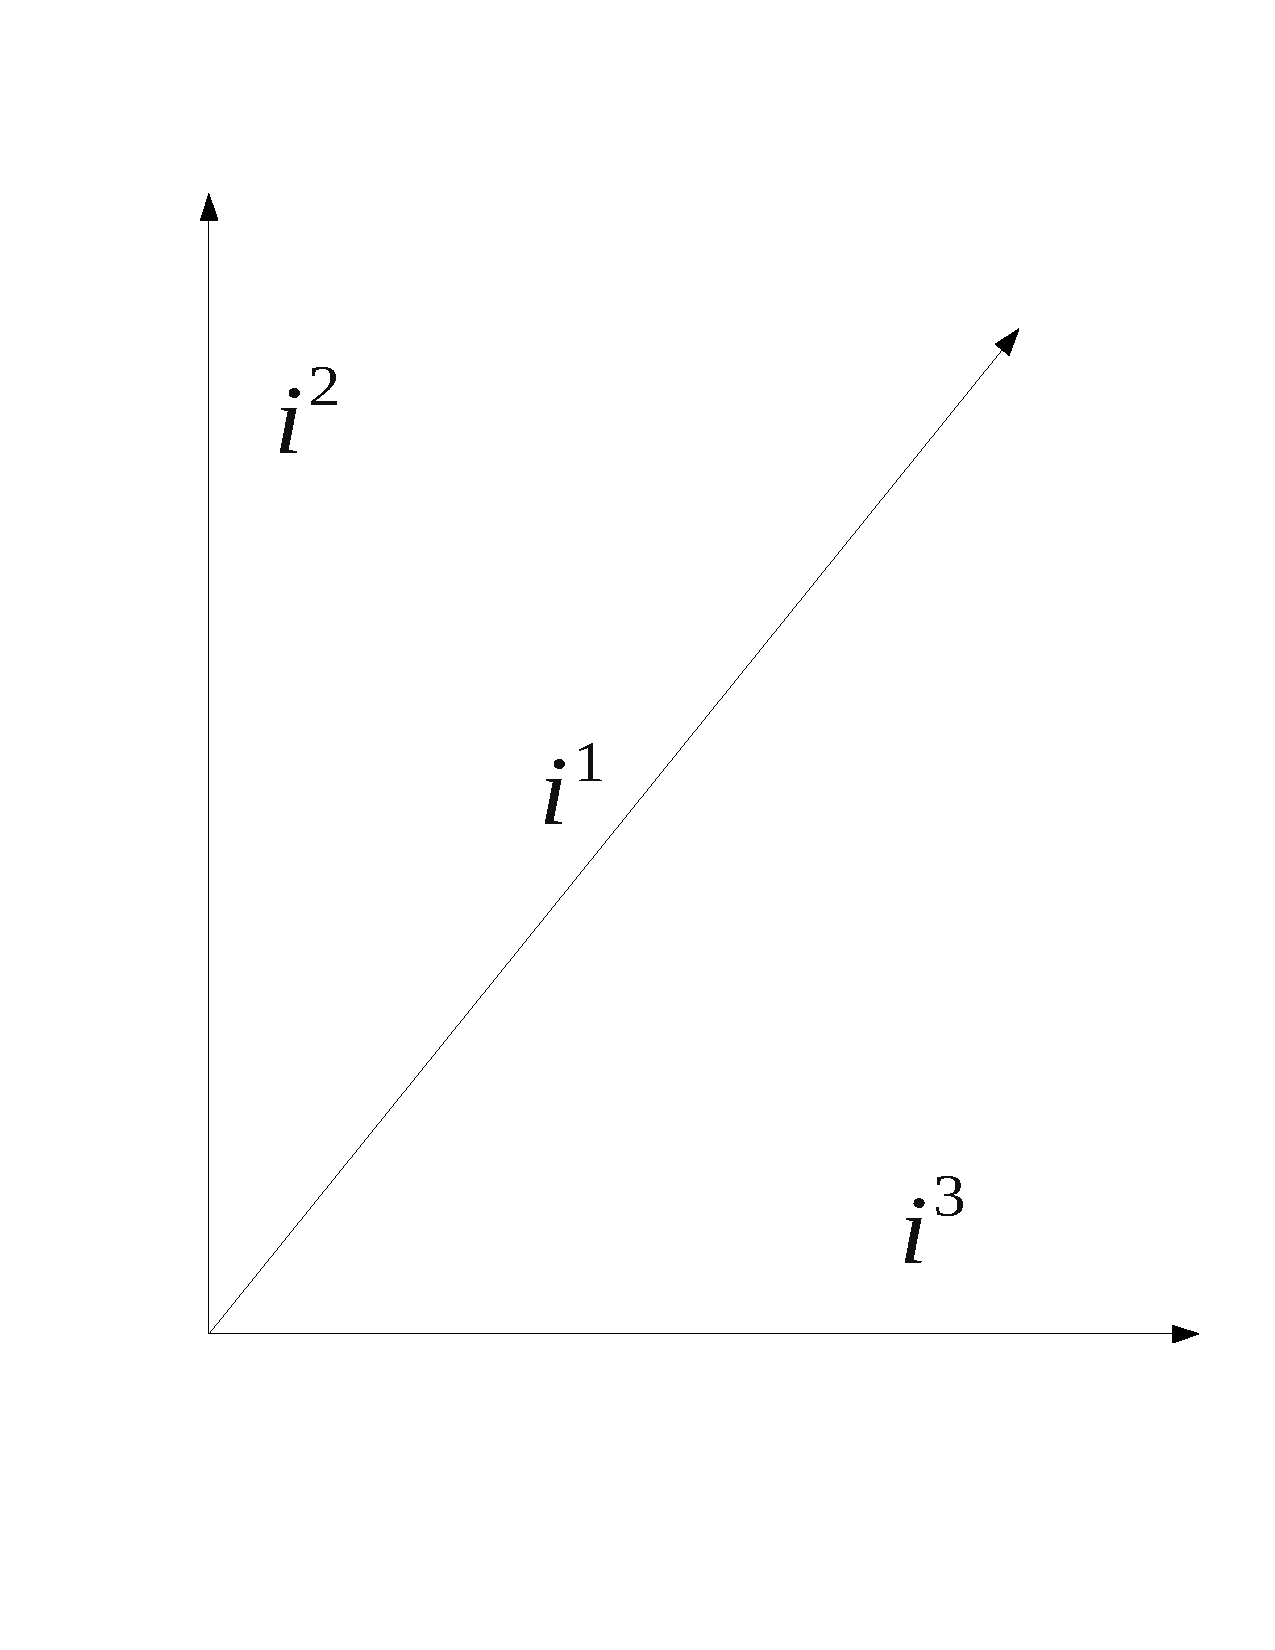
\includegraphics[width=4in,height=3in]{pics/cos-trans-pic.pdf}
\end{center}
\label{fig:no-cos-trans}
\end{figure}

Казалось бы, что значение $\Delta_i = 0,5$ слишком мало, и надо требовать, чтобы
оно стремилось к 1, как было показано на рисунке <<Нарушение транзитивности при использовании меры сходства косинус>> (\ref{exmpl:non-trans-cos}).
Однако такое значение $\Delta_i$ может удовлетворять
реальной РС.
Например, рассмотрим ситуацию, которая может быть характерна
для компании Amazon \cite{amazon-item2item}: объектами являются векторы в
пространстве пользователей, то есть $Y = U, c_Y(i) = (w(1),..,w(m))$
\begin{equation*}
	w(u) =
  \begin{cases}
	1, &\text{если $u \R i$ (пользователь приобрел товар $i$)}\\
	0, &\text{иначе}.
  \end{cases}
\end{equation*}
Данной системой пользуется огромное число человек, поэтому ситуация,
когда товар приобрели, к примеру, 100000 человек, возможна, и вполне
уместно считать товары $i,j$ схожими, если их приобрели более,
чем 49000 одних и тех пользователей.

Для СОМ характерной функцией меры сходства является корреляции Пирсона при
представлении контента пользователя $u$ как выборки
$\{\rho(u,i_0)\}$.

 \begin{equation}
  \du(u, v) =
h \frac{\sum \limits_{i_0 \in P^u_0 \bigcap P^v_0}
	(\rho(u,i_0) - \overline{\rho^u}) \cdot
	(\rho(v,i_0) - \overline{\rho^v})}
	{\sqrt{\sum \limits_{i_0 \in P^u_0}(\rho(u,i_0) -
	\overline{\rho^u})^v \sum \limits_{i_0 \in
	P^v_0}(\rho(v,i) - \overline{\rho^v})^v}}
\end{equation}
В общем случае (при $\Delta_u \in [0,1]$, а не только $\Delta_u = 1$)
коэффициент корреляции не обладает свойством транзитивности
\cite{pearson-trans}, и поэтому в общем случае при применении
данной функции в качестве меры сходства достаточное и необходимое условия не
выполняются.

Если транзитивность в кластере соседей не выполняется, то это приводит
к возрастанию погрешности прогнозной оценки,
так как оценки соседей на прогнозируемый объект могут сильно разниться.

Например, $a = (0,7; 1; 0,1; i_{\bot})$, $u = (0,65; 0,9; 0,1; 1)$,
$v = (0,73; 0,95; 0,05; 0,1)$, $\Delta_u = 0,9$.
Тогда $\du(u_a, u) = 0.9997$, $\du(u_a, v) = 0.9953$, то есть пользователи
$u, v$ попадают в кластер соседей, будучи несхожими
$\du(u, v) = 0.46$. А оценка на неизвестный объект $i_{\bot}$ составляется
из совершенно разных оценок $1$ и $0,1$.
\subsection{Вывод}
Эффективность по критерию качества при применении АКМ для решения задач
зависит от разработчика, а именно от выбора им функционального и тестового
параметра. Не всегда возможно подобрать
функциональный и пороговый параметры так, чтобы выполнялись условия
эффективности решения и реализация РС соответствовала требования
заказчика как, например, в вышеописанном примере для ООМ и $\Delta_u = 0,5$.
АКМ не являются эффективными по критерию качества.
%%%%%%%%%%%%%%%%%%%%%%%%%%%%%%%%%%%%%%%%%%%%%%%%%%%%%%%%%%%%%%%%
%%%%%%%%%%%%%%%%%%%%%%%%%%%%%%%%%%%%%%%%%%%%%%%%%%%%%%%%%%%%%%%%
%%% SPLIP: свойства
%%%%%%%%%%%%%%%%%%%%%%%%%%%%%%%%%%%%%%%%%%%%%%%%%%%%%%%%%%%%%%%%
%%%%%%%%%%%%%%%%%%%%%%%%%%%%%%%%%%%%%%%%%%%%%%%%%%%%%%%%%%%%%%%%
\section{Эффективность по критерию стабильности}
\subsection{Истинность правил вывода}
Правила вывода АКМ, основаны на эвристических
утверждениях. Существующие исследование не анализируют выполнимость этих
утверждений, правила вывода носят аксиоматический характер. Однако,
выполнение эвристических утверждений зависит от свойств исходных данных.
Рассмотрим свойства исходных данных и их влияние на выполнение утверждений.
\subsubsection{Динамика}
В реальности РС работают с динамической информацией,
которая постоянно меняется во времени:
меняется популярность объекта и его восприятие пользователями,
а мощности $U, I$ постоянно растут.
К примеру, новостная система Google News \cite{google-news} ежедневно
пополняет множество объектов, которые являются новостями.

Так же с течением времени меняются потребности и предпочтения пользователей,
поэтому периодически необходимо производить пересмотр их предпочтений \cite{changes}.

Рассмотрим влияние на каждый тип АКМ свойства динамики данных:
\begin{itemize}
	\item утверждение (\ref{assertORS1}) и решение задачи $topN$:
		$(u_a \rt i_0) \wedge (i_0 \rt i) \Rightarrow u_a \R i$.
		Если с течением времени и смене вкусов пользователя меняется отношение
		пользователя к объектам $i_0$ так, что $\rho(u_a,i_0) < \Delta_{\R}$,
		то и $\rho(u_a,i) < \Delta_{\R}$, так как $i_0 \rt i$.
		Таким образом, не выполнится отношение $u_a \R i$, входящее
		в эвристическое утверждение (\ref{assertORS1}), и тогда
		$\eat > \varepsilon_{topN}$, так как цель,
		поставленная при решении задачи $topN$ не будет достигнута. В
		результирующее множество будут входить такие объекты, между которыми и
		активным пользователем не выполняется отношение близости, то есть
		решение неэффективно.

		К примеру, РС интернет-магазина одежды располагает
		данными о покупках пользователя, совершенных зимой. Прибегая к помощи
		системы весной, пользователь, скорее всего, получит в качестве рекомендаций
		зимнюю одежду, хотя планирует выбрать летнюю;

	\item Утверждение СОМ гласит: если в прошлом пользователи были близки по вкусам,
		то и в будущем они будут близки по вкусам. Однако, учитывая динамику
		пользователей, предпочтения пользователей могут смениться так, что
		отношение близости не будет выполняться.

		Если решение будет построено на основании данных некоторого кластера
		$\nup$, и с течением времени предпочтения сменились так, что
		для некоторых $u \in \nup$: $\du(u_a, u) < \Delta_u$, то при
		формировании решения на таком кластере оно будет неэффективным по
		критерию качества, так как нарушится необходимое
		(\ref{suf-cond-pred-srs}) и достаточное (\ref{nec-cond-pred-srs})
		условие: транзитивность отношения близости на кластере.
		Поэтому нужно заново выполнять построение
		кластера, что неэффективно по критерию вычислительной сложности:
		гораздо эффективней единожды сформировать кластер и работать в дальнейшем с
		ним.
\end{itemize}

Таким образом, имеет место быть следующее утверждение.
\begin{assert}
	\label{ass:dynamic}
Если для исходных данных характерно свойство динамики, то
эвристические утверждения могут не выполняться для любого активного
пользователя. И, как следствие, истинность правил вывода нарушается, а решение,
полученные на их основе не являются эффективными по критерию качества решения.
\end{assert}
%Однако, данные, которые были изменены и, тем самым, ухудшают качественность
%результата, могут системой не рассматриваться.
%Если такая информация составляла бОльшую часть контентов,
%то может возникнуть проблема разреженности данных\cite{sparse1, sparse2,
%sparse3}.
%
%Помимо этого, постоянное пополнение множества объектов ведет к проблеме
%добавления нового элемента, следствием
%которого является пересчет матрицы оценок сходства объектов, что, с точки
%зрения вычислительных затрат, является
%дорогим процессом. К примеру, в системе, где есть миллион объектов,
%для добавления нового объекта нужно провести
%миллион операций вычисления оценки сходства.

\subsubsection{Неоднородность предпочтений}
Предпочтения пользователей {\it неоднородны} \cite{psy, hetero-spotify,hetero1}, что означает, что
пользователь может предпочитать совершенно различные объекта, которые не
обязательно являются соседями:
\begin{assert}\label{neodnorodost}
$(u_a \R i) \wedge (u_a \R j) \not \Rightarrow (i \rt j)$.
\end{assert}

Из того, что выполняется $(u_a \R i_0) \wedge (u_a \R i_{\bot})$
нельзя утверждать, что выполняется $i_0 \rt i_{\bot}$, так как значение
$\du(i_0, i_{\bot})$ может быть как больше $\Delta_u$, так и меньше,
в силу того, что вкусы пользователя неоднородны.

К примеру, для кинематографической РС, где характеристиками объектов
являются кинематографические жанры, пользователю могут нравиться как фильм
ужасов $i_0$, так и комедия $i_{\bot}$. Тогда
$(u_a \R i_0) \wedge (u_a \R i_{\bot})$
$\cancel{\Rightarrow} i_0 \rt i_{\bot}$,
так как по кинематографическим жанрам объекты $i_0$ и $i_{\bot}$ не являются
близкими.

Рассмотрим влияние данного свойства:
\begin{itemize}
	\item Рассмотрим ООМ и задачу $topN$. Пусть $P^a_0 = \overline{P}^a_0
		\bigcup \underline{P}^a_0$, где $\overline{P}^a_0$ такое, что $\forall
		i_0,j_0: i_0 \rt j_0, \rho(u_a, i_0), \rho(u_a, j_0) \in
		\overline{P}^a_0$.
		$\underline{P}^a_0$ такое, что $\forall k_0: \di(i_0, k_0) \le \Delta_i$,
		$\rho(u_a, i_0) \in \overline{P}^a_0, \rho(u_a, k_0) \in \underline{P}^a_0$
		Решение (\ref{alg:topn-solve-ors}), реализованное при помощи правила
		вывода ООМ (\ref{ors-pi-top}), применяемым для задачи $topN$
		, будет иметь
		вид $I_{topN} = \{ i: i_0 \rt i \}$,
		если $|\overline{P}^a_0| > |\underline{P}^a_0|$.
		Но тогда в решении существуют две проблема:
		\begin{enumerate}
			\item Рекомендация получается \lq однотипной\rq, так как в
				результирующее множество не попадают объекты, соответствующие
				предпочтениям, которые характерны для объектов типа $k_0$;
			\item Если $P^a_{\bot} = \{ i_{\bot} | k_0 \rt i_{\bot}
				\}$, то вышеприведенное решение будет неэффективным по критерию
				качества $\eit$,
				так как $\eit \rightarrow 1$.
		\end{enumerate}

	\item Рассмотрим CОМ и задачу $pred$.
	Рассмотрим пример данных о пользователе из предыдущего пункта.
	Возможна ситуация, когда
	для такого активного пользователя с неоднородными данными будет составлено
	множество соседей $\{u,v\}$ с односторонними предпочтениями.
	Для пользователя $u$ входное множество данных будет иметь вид
		$\{i_0, u_a, \rho(u_a, i_0)\}: \rho(u_a, i_0) > \Delta_{\R} \}$
		$\bigcup$
		$\{j_0, u_a, \rho(u_a, j_0)\}: \rho(u_a, i_0) = 0 \}$
	Для пользователя $v$ входное множество данных будет иметь вид
		$\{i_0, u_a, \rho(u_a, i_0)\}: \rho(u_a, i_0) = 0 \}$
		$\bigcup$
		$\{j_0, u_a, \rho(u_a, j_0)\}: \rho(u_a, i_0) > \Delta_{\R} \}$

	Пусть $\du = \cos$, тогда возможна ситуация, когда $\du(u, v) = 0$, то есть отношение
	близости $u \ru v$ не выполняется, и поэтому
	нарушается необходимое (\ref{nec-cond-pred-srs}) и
	достаточное (\ref{suf-cond-pred-srs})
	условие эффективного решения по критерию качества.
	\end{itemize}

\begin{assert}
	\label{ass:hetero}
Если для исходных данных характерно свойство неоднородности, то
эвристические утверждения могут не выполняться для любого активного
пользователя. И, как следствие, истинность правил вывода нарушается, а решение,
полученные на их основе не являются эффективными по критерию качества решения.
\end{assert}

Следует отметить, что ООМ, в основном, применяется для задачи $topN$, тогда как
СОМ --- для задачи $pred$. Было показано, что если данные обладают
свойством динамики и неоднородности, то ООМ и СОМ не гарантируют получение
качественного решения.



\subsection{Вывод}
Получение эффективного решения по критерию качества при применении
АКМ зависит от свойств исходных данных, поэтому
\begin{assert}
	\label{input-props-kf}
	АКМ неэффективны по критерию стабильности.
\end{assert}



%Рассмотрим доказательство в более простом случае ---
%при применении средней близости для вычисления
%неизвестного $\rho(u_a,i_{\bot})$\cite{middle-pred}
%$\overline{\rho}(u_a,i_{\bot}) = \frac{1}{|\nup|} \sum
%\limits_{u \in \nup} \rho(u,i_{\bot})$
%, где $\overline{\rho}(u_a,i_{\bot})$ ---
%спрогнозированная близость.
%
%Рассмотрим доказательство для случая, когда $\nup = \{u,v\}$.
%%Пусть $\rho(u_a, i_{\bot}) \ge \overline{\rho}(u_a,i_{\bot})$, тогда
%%% Тут я просто снял модуль и расписал среднее для двух соседей
%%$\rho(u_a,i_{\bot}) - \frac{1}{2}\cdot(\rho(u,i) + \rho(v,i))$.
%Так как $u_a \ru u$, то $|\rho(u_a, i_{\bot}) - \rho(u,i_{\bot})| \le \varepsilon_p$
%по определению \ref{user-sim1}.
%Тогда $\rho(u,i_{\bot}) - \varepsilon_p \le \rho(u_a,i_{\bot}) \le \varepsilon_p +
%% от тут просто подставляю ро(а,и) в исходную разность
%\rho(u,i_{\bot})$. Оценим разницу $A = \rho(u_a,i_{\bot}) -
%\frac{1}{2}\cdot(\rho(u,i) + \rho(v,i))$:\\
%$\frac{1}{2} \cdot (\rho(u,i_{\bot}) - \rho(v, i_{\bot})) \varepsilon_p \le A
%\le \frac{1}{2} \cdot (\rho(u,i_{\bot}) - \rho(v, i_{\bot})) + \varepsilon_p$.
%
%Оценим разность
%$|\rho(u_a,i_{\bot}) - \overline{\rho}(u_a,i_{\bot})| = |\rho(u_a,i_{\bot}) -
%\frac{1}{|\nup|} \sum \limits_{u \in \nup} \rho(u,i_{\bot})|$.
%Так как $u_a \ru u$, то по определению \ref{user-sim1}
%$|\rho(u_a,i_{\bot}) - \rho(u,i_{\bot})| \le \varepsilon_p$, а, значит,
%$\frac{1}{2} \cdot (\rho(u,i_{\bot}) - \rho(v,i_{\bot}) \varepsilon_p
%\ge |\rho(u_a,i_{\bot}) - \overline{\rho}(u_a,i_{\bot})|
%\le \frac{1}{2} \cdot (\rho(u_a,i_{\bot}) - \rho(v,i_{\bot})) + \varepsilon_p$.
%Так как $|\rho(u_a,i_{\bot}) - \overline{\rho}(u_a,i_{\bot})| \le \epsilon_p$,
%то $\rho(u,i_{\bot}) - \rho(v,i_{\bot} \le 2\cdot \epsilon_p +
%2 \cdot \varepsilon_p$


%%%%%%%%%%%%%%%%%%%%%%%%%%%%%%%%%%%%%%%%%%%%%%%%%%%%%%%%%%%%%%%%
%%%%%%%%%%%%%%%%%%%%%%%%%%%%%%%%%%%%%%%%%%%%%%%%%%%%%%%%%%%%%%%%
%%%% SPLIP: применимость етоп
%%%%%%%%%%%%%%%%%%%%%%%%%%%%%%%%%%%%%%%%%%%%%%%%%%%%%%%%%%%%%%%%
%%%%%%%%%%%%%%%%%%%%%%%%%%%%%%%%%%%%%%%%%%%%%%%%%%%%%%%%%%%%%%%%

%\subsection{Необходимое и достаточное условия объективного применения оценок
%эффективности задачи $topN$ при использовании ООМ}
%%% ООМ основаны на эвристических утверждениях, которые выносят предположение относительно
%%% оценки сходства  пользователя и объекта, исходя из схожести только объектов и без введения
%%% соответствующей оценки сходства с область определения $U \bot P$. Это и является основной причиной проблем, которые будут описаны.
%%% Вместо того, чтобы производить непосредственно рассчет $\delta(u_a,i_{\bot})$ РС производят косвенные рассчеты, в основу которых
%%% заложена недоказуемая эвристика.
%Напомним, что целевая задача $topN$ состоит в построении $I_{topn} = \{i: u_a
%\R i\}$.
%Таким образом, по отношению к задаче $topN$, решение
%эффективно по критерию качества, если
%\begin{equation*}
%|\{ i \in \overline{P}^a_{\bot} |u_a \R i \}| = K \ge N \cdot (1 - \varepsilon_{topN})
%\end{equation*}
%Однако, для ООМ проверка выполнения условия $u_a \R i$ основана на
%эвристическом утверждении ООМ \ref{assertORS1}.
%Чтобы показатель $\eit$ соответствовал целевой задаче, нужно, чтобы
%если решение является эффективным по $\eit$, то решение являлось бы эффективным
%и по $\eat$, и наоборот.
%
%То есть должны выполняться следующие два условия:
%\begin{equation}\label{etop-use1}
%\eit \le \varepsilon_{topN} \Rightarrow \eat \le \varepsilon_{topN}
%\end{equation}
%и
%\begin{equation}\label{etop-use2}
%\eat \le \varepsilon_{topN} \Rightarrow \eit \le \varepsilon_{topN}
%\end{equation}
%
%Проанализируем выполнение \ref{etop-use1}.
%Если решение качественно по $\eit$, то
%$\exists I^{\prime}_{topN} \subset I_{topN}, I^{\prime}_{topN} = \{i: \exists
%i_{\bot}, i \rt i_{\bot} \}, |I^{\prime}_{topN}| = K > N \cdot (1 - \varepsilon_{topN}$
%По данным задачи выполняется
%$u_a \R i_{\bot}$, а по решению --- $i \rt i_{\bot}$,
%поэтому, если выполняется утверждение ООМ \ref{assertORS1}, то выполняется отношение
%$u_a \R i$ для $i \in I^{\prime}_{topN}$,
%и тогда значение $\eat < \varepsilon_{topN}$, то есть решение эффективно по критерию
%качества.
%
%Проанализируем выполнение (\ref{etop-use2}). Так как решение эффективно по
%$\eat$, то
%$\exists I^{\prime}_{topN} \subset I_{topN}, I^{\prime}_{topN} = \{i: u_a \R
%i\}, |I^{\prime}_{topN}| = K > N \cdot (1 - \varepsilon_{topN}$
%По данным задачи и по решению известно, что:
%\begin{equation} \label{ors-cond}
%	(u_a \R i_{\bot}) \wedge (u_a \R i)
%\end{equation}
%
%Учитывая утверждение ООМ \ref{assertORS1} и \ref{ors-cond},
%на первый взгляд можно предположить
%выполнение транзитивности отношения близости:
%$\Big((u_a \R i_{\bot}) \wedge (u_a \R i) \Big)  \Rightarrow (i \rt i_{\bot})$.
%Однако утверждение \ref{neodnorodost} показывает, что $ik \rt i_{\bot}$
%может не выполняться при выполнении \ref{ors-cond}.
%Поэтому, если решение качественно по целевой оценке,
%оно может быть {\it неэффективно по оценке} $\eit$, если
%$i \in I^{\prime}_{topN}$, $\du(i, i_{\bot}) \le \Delta_u$ и $|I^{\prime}_{topN}|
%\rightarrow N$, что возможно в силу
%неоднородности предпочтений пользователя.
%
%\begin{assert}
%\label{eit-use}
%Оценка $\eit$ может применяться для определения качества
%решения задачи $topN$ методами ООМ, если выполняется эвристическое утверждение ООМ
%	(assertORS1),
%	что зависит от
%исходных данных.
%\end{assert}

\section{Эффективность по критерию вычислительной сложности}
Вычислительную сложность будем характеризовать асимптотической сложностью
решений, а в качестве элементарной операции возьмем операцию вычисления
значения меры сходства (общую операцию, выполнение которой необходимо для
решения любой задачи при применении любого из правил вывода).

Так как $\Pi_O$ применяется, в основном, для решения задачи $topN$, а
$\Pi_C$ для решения задачи $pred$, то будем рассматривать
асимптотические сложности алгоритмов только для таких случаев.

Асимптотическая сложность алгоритма решения задачи $topN$ при применении
$\Pi_O$ равна $O(n^2)$.
Асимптотическая сложность алгоритма решения задачи $pred$ при применении
$\Pi_C$ равна $O(m)$.

Учитывая огромные мощности множеств $U$ и $I$ при работе реальных РС
с реальными данными и обозначенные асимптотические сложности, для АКМ
имеет место быть проблема масштабируемости \cite{amazon-item2item}, а потому АКМ неэффективны по
критерию вычислительной сложности.

\section{Цели и задачи исследования}
Анализ АКМ выявил следующие открытые проблемы:
		\begin{enumerate}
		\item решение задачи эффективно по критерию качества,
			если выполняются
			эвристические утверждения, что зависит от свойств исходных данных.
			В общем случае, получение качественного решения при применении АКМ
			не гарантировано;
		\item качество решения при применении АКМ зависит
			от следующих параметров системы, которые выбираются разработчиками:
				\begin{enumerate}
					\item функции, которая применяется в качестве меры сходства
				$\du$ для СОМ, $\di$ для ООМ;
		\item порогового значения $\Delta_i, \Delta_u$.
				\end{enumerate}
		\item проблема масштабируемости
		\end{enumerate}

%Цель исследования --- разработка математической модели РС, в которой можно
%более эффективно применять $\Pi_O$ и $\Pi_C$, и определение методов решений во
%введенной модели, не уступающих по эффективности коллаборативным.
%
%Для достижения цели решим следующие задачи:
%\begin{enumerate}
%		\item ввести формальные термины и математические обозначения, в которых определить
%			задачи рекомендательных систем, коллаборативную модель и методы решений
%			задач;
%
%		\item определить критерии оценки эффективности модели и показать, что
%			коллаборативная модель не является эффективной моделью
%			по качеству решения, стабильности и вычислительной сложности;
%
%		\item разработать математическую модель РС, в которой
%
%		\begin{enumerate}
%			\item определить формальные правила вывода, не основанные на
%				эвристических утверждениях;
%			\item определить алгоритмы решения задач, не менее эффективные по
%				по сравнению с алгоритмами
%				коллаборативной модели.
%		\end{enumerate}
%
%	\item реализовать программное обеспечение на основе разработанной модели
%		для демонстрации практического применения разработанной модели;
%
%	\item реализовать программное обеспечение для проведения тестирования
%		коллаборативной и разработанной моделей.
%\end{enumerate}
%
